\chapter{Proposed Solution}
\section{Solution Overview and ROS 2 System Model}
The proposed solution follows a hybrid architecture that combines deterministic ROS~2 system analysis with large language model reasoning. The deterministic part establishes what exists in the robot software, how it is deployed, where its configuration values originate, and which concrete locations can be modified. The language-model part interprets the meaning of a user request, identifies the configuration elements relevant to that request, and proposes new values. A final deterministic boundary validates and applies the proposal. This separation is fundamental: objective repository facts are extracted rather than guessed, while semantic decisions that cannot be done deterministically are assigned to the language model.
The method operates at two distinct steps. First, at artifact-generation time, the ROS~2 project is analyzed and converted into a representations made of multiple JSON files. These representations include the integrated deployed-system model, the physical configuration space, grounded parameter evidence, rendering templates, a complete baseline configuration, and the relationships required to reason about ROS interfaces. Second, for each user request, the system performs capability interpretation, parameter retrieval, parameter selection, value reasoning, deterministic validation, and configuration application.
Separating these time scales prevents the system from rediscovering the repository during every interaction. The source repository is treated as the authority from which deterministic knowledge is generated. Once generated and validated, that knowledge becomes an immutable source of truth until the repository or the extraction method changes and the artifacts are deliberately regenerated. By doing this, multiple language-model experiments can be performed against exactly the same representation of the robot. The complete method consists of the following stages:

\begin{enumerate}
    \item deterministic extraction of ROS~2 source, deployment, and configuration facts;
    \item integration of those facts into a unified deployed-system model;
    \item projection of all discovered launch arguments and ROS parameters into a physical configuration representation;
    \item construction of bounded, traceable evidence for every configuration element;
    \item interpretation of the user request in terms of supported robot capabilities;
    \item deterministic realization of the selected capabilities and verification of required ROS connections;
    \item deterministic retrieval of a bounded set of relevant ros nodes;
    \item language-model selection of the relevant parameters and separate reasoning about their new values;
    \item deterministic generation, validation, and application of a sparse configuration plan.
\end{enumerate}

\begin{figure}[htbp]
    \centering
    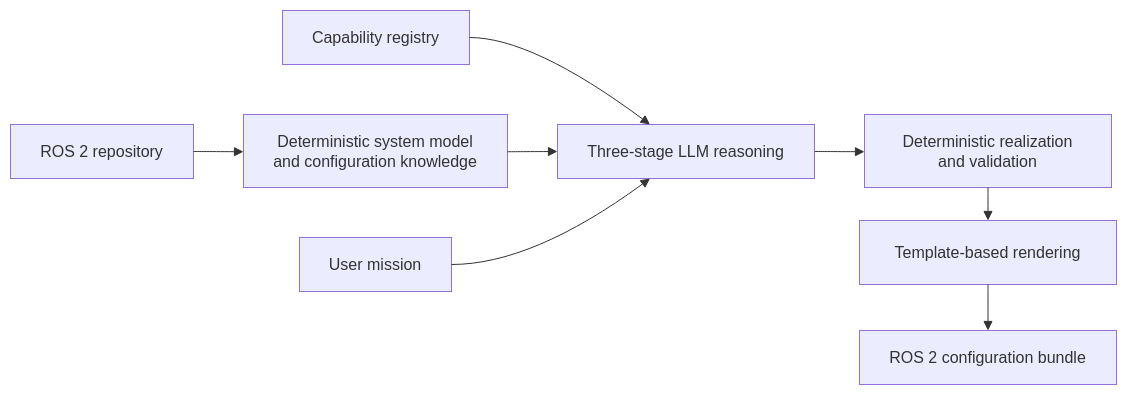
\includegraphics[width=0.96\textwidth]{pics/diagram1.png}
    \caption{Complete architecture of the proposed hybrid ROS~2 configuration framework.}
    \label{fig:proposed-complete-architecture}
\end{figure}

The proposed solution deliberately does not allow the language model to write arbitrary launch or parameter files. The model operates through structured contracts whose outputs refer to identifiers already present in the frozen configuration representation. Launch and YAML artifacts are produced only after the proposed identifiers and values have passed deterministic checks. In this way, language-model reasoning is used where semantic interpretation is required, while conventional software remains responsible for existence, type, provenance, consistency, and rendering correctness.

The first methodological requirement is to construct trustworthy knowledge about the ROS~2 project. A natural-language request cannot be mapped reliably to configuration changes if the reasoning process does not know which nodes exist, which parameters they consume, how they communicate, or which deployment path is active. The extraction stage treats the repository as a source of evidence rather than as a collection of isolated files.
Python source analysis identifies ROS-specific entities declared by the application. The extracted information includes nodes, declared parameters, parameter reads, publishers, subscriptions, services, clients, actions, timers, quality-of-service descriptions, and transform-related operations. Source locations and unresolved expressions are retained rather than discarded. This is important because later reasoning must distinguish a directly observed fact from an expression that could not be resolved statically.
Each category contributes different grounding information. A declared parameter identifies a possible control point. A parameter read and its surrounding usage provide evidence about behavioral effect. Publishers and subscriptions show how a component participates in the system and the dependency relationship with other components. Message types constrain whether two endpoints can communicate. Quality-of-service information allows the method to detect known incompatibilities.
The purpose of source analysis is not to reconstruct arbitrary Python execution perfectly. Its role is to recover a bounded set of objective ROS facts sufficient to ground configuration reasoning. When a value depends on dynamic computation or an unsupported Python pattern, the method records the unresolved expression instead of fabricating a result.
Source-level node declarations do not by themselves describe the deployed robot. ROS~2 launch descriptions determine which executables are instantiated, which namespaces and node names become effective, which conditions enable or disable them, and how launch arguments flow through included launch files. The method therefore extracts launch declarations, include relationships, launch arguments, substitutions, parameter sources, remappings, namespaces, conditions, package names and executable names.
Launch arguments are retained as configuration elements because they often control whether a subsystem is active or which implementation is selected. Conditions are preserved because the presence of a node in source code does not imply that it is enabled in the current baseline. Remappings and namespaces are resolved because communication compatibility depends on effective ROS names, not merely on the literals appearing in individual source files.
ROS parameter files provide another layer of configuration. The method extracts node selectors, nested parameter paths, scalar and structured values, and the provenance of each assignment. Wildcard selectors require special treatment. A wildcard assignment may configure several deployed nodes, but it still corresponds to one writable location in the source configuration file. The method records every affected component while preserving the fact that the value is controlled by one physical slot.
Parameter-file extraction also captures the relationship between declared defaults and deployment-time values. A parameter may have a default in Python, an assignment in YAML, and an additional launch-level source. Retaining these layers makes it possible to determine both the effective value and the location that must be modified. The output of extraction is a structured collection of observed facts, resolved values, provenance links, and explicit unresolved information.

The extracted sources describe overlapping views of the same robot. Python analysis describes possible node behavior, launch analysis describes deployment, parameter files describe configuration assignments, and package metadata describes software boundaries. The integration stage combines these views into one coherent representation of the deployed system.
The central unit of the integrated model is the deployment instance. A deployment instance connects a launch-level node action to its source-level node representation when the source is available. It records the effective node name, namespace, package, executable, activation condition, source reference, parameter sources, interfaces, and resolution status.
The distinction between a source component and a deployment instance is important. One source component may be instantiated more than once, under different names or namespaces, or may remain disabled under the selected root launch. On the other hand, a launch description may instantiate an external component for which no local source model exists. The integrated representation retains both cases.
Configuration values can originate from several layers. The method retains the declared default, YAML assignment, launch-provided parameter source, root override, and final effective value whenever those layers are available. Rather than storing only the final number or string, the model stores the ordered provenance that produced it.
Provenance has two roles. First, it supports traceability: a proposed change can be connected to the source or configuration location that controls it. Second, it supports correct application: modifying a Python default that is located inside the node definition is not equivalent to modifying a YAML assignment that overrides that default in the deployed system. The method must target the controlling physical location rather than the earliest declaration encountered during extraction.
Publishers, subscriptions, services, and other ROS entities are projected into the deployment context. Namespaces and remappings are applied to obtain effective interface names. Where sufficient local evidence exists, compatible publisher--subscription pairs are represented as confirmed communication edges. The model retains endpoint role, effective name, interface type, owning component, and available quality-of-service information.
Only relationships supported by evidence are asserted. When an endpoint belongs to an external package whose source cannot be inspected, the method records partial knowledge rather than assuming a complete connection. This conservative treatment is essential because the unified model later serves as evidence for both deterministic validation and language-model reasoning.
Every deployment instance and relationship carries an explicit resolution status. Locally resolved instances have source evidence and known extracted interfaces. External instances are represented as deployed components with unknown internal behavior. Partial or unresolved launch expressions are collected in a dedicated set of unresolved facts.
Uncertainty is therefore represented in the data. Later stages can distinguish a confirmed missing connection from one that cannot be verified because an external component has an unknown implemententation. This prevents the system from reporting certainty where the repository does not provide it.
The integrated model describes effective parameter occurrences, but configuration application requires writable physical locations. These two concepts are not always one-to-one. The method therefore projects the system model into a configuration representation whose records correspond to physical launch arguments and ROS parameter slots.
Each configuration record retains a stable identifier, source name, kind, value type, default value, current effective value, allowed values or known numerical bounds when available, provenance, modification targets, affected components, and relationships to other records. Every discovered physical slot is included as a potential configuration candidate. The method does not use a manually maintained permission policy that classifies parameters as configurable or fixed.
This design allows hardware dimensions, algorithm settings, topic names, frame identifiers, timing parameters, and launch arguments to participate in the same reasoning process. Their semantic categories may differ, but category membership does not determine whether the user is allowed to request a change. Relevance is determined for each mission, while objective validity is checked later.
When one wildcard YAML value affects multiple components, the representation contains one configuration record with multiple affected components. This prevents the reasoning process from proposing contradictory values for aliases that ultimately write to the same location.
The integrated model and the physical configuration representation are saved as frozen artifacts. Here, frozen means that they are treated as immutable inputs for a run or experiment. It does not refer to a ROS runtime feature. When source code, launch structure, parameter files, or extraction logic changes, the dependent artifacts must be regenerated in order.
This frozen boundary makes the language-model experiment reproducible. The same identifiers, values, relationships, and evidence can be supplied across repeated runs and context ablations.

\begin{figure}[htbp]
    \centering
    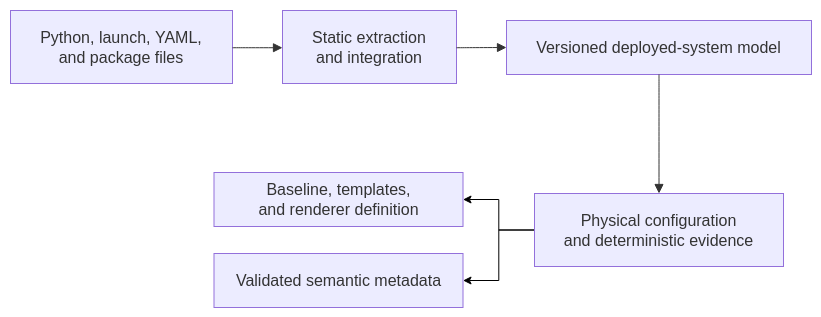
\includegraphics[width=0.90\textwidth]{pics/det_knowledge_artifact_generation.png}
    \caption{Deterministic construction of system knowledge and configuration artifacts.}
    \label{fig:deterministic-knowledge-generation}
\end{figure}

\section{Deterministic Evidence and LLM-Enriched Parameter Metadata}
Metadata is constructed for every writable physical configuration slot discovered in the analyzed deployment. The current method combines two deliberately separated sources. Deterministic repository analysis establishes parameter identity, type, current value, provenance, writable target, affected components, source evidence, and relationships directly supported by the analyzed system. A separate language-model enrichment stage derives semantic descriptions and vocabulary that are difficult to recover through syntax alone. The semantic enrichment never replaces the deterministic identity or evidence of a parameter and cannot introduce a new writable configuration slot.
The construction starts from effective parameter occurrences in the unified system model. Occurrences controlled by the same physical location are grouped into one configuration record. A ROS parameter assigned through YAML is identified by its file, node selector, and nested parameter path. A launch argument is identified by its root launch interface. This projection is necessary because one YAML wildcard may affect several deployed components, whereas configuration application must still modify that value only once.
For each resulting record, the deterministic extractor assigns a stable canonical identifier and retains the source name, configuration kind, value type, declared default, current effective value, known allowed values or numerical bounds, ordered provenance, writable target, affected components, and deterministically discovered relationships. It also creates a bounded evidence package containing source references and short excerpts for declarations, reads, and usages, together with related ROS interfaces when those interfaces can be established from the repository. Unavailable deterministic facts remain absent or explicitly unresolved; they are not inferred from the parameter name.

The semantic-enrichment model receives the bounded evidence document for one parameter per request. For each document it may produce a concise description, aliases, example user expressions, physical quantity, unit, semantic category, behavioral effects, constraints, typed relationships to other known parameters, and a confidence value. Processing one parameter at a time keeps the prompt within the configured 8192-token context and prevents the response for one parameter from being confused with another. Every response is schema-validated and saved immediately to an incremental checkpoint, so an interrupted run resumes from the last completed parameter. The frozen enrichment used in the present experiments contains one validated record for each of the 109 configuration entries. At the request of the experimental design, evidence identifiers are not required from the enrichment model and are stored as empty lists; the semantic fields must therefore be treated as uncited model-generated hypotheses rather than as source quotations. Schema validation still prevents invented parameter identities and invalid relationship targets. The enrichment artifact is hash-bound to the system model and configuration schema, so stale metadata is rejected at application start-up. Once a validated enrichment artifact is frozen for an experiment, retrieval over the combined records is reproducible even though the offline process that originally generated the semantic hypotheses used a language model.

Table~\ref{tab:deterministic-parameter-metadata} illustrates the combined record for one parameter and identifies the origin of each group of fields. The deterministic part shows why both provenance and a writable target are required: the node declares a default of \(10.0\), but the deployed YAML assignment overrides it with \(20.0\). Consequently, \(20.0\) is the current effective value and the YAML slot is the location that configuration generation must modify. The language-model part adds searchable ways of expressing the same parameter semantically, while remaining subordinate to the source-derived identity, value, target, and evidence.

\begin{table}[htbp]
\centering
\caption{Example of combined deterministic and language-model-generated metadata for a ROS parameter.}
\label{tab:deterministic-parameter-metadata}
\begin{tabular}{p{0.27\textwidth} p{0.66\textwidth}}
\hline
\textbf{Metadata field} & \textbf{Extracted value} \\
\hline
\multicolumn{2}{l}{\textit{Deterministically extracted facts and evidence}} \\
Canonical identifier & \texttt{nodes.joint\_state\_estimator.publish\_frequency} \\
Source parameter name & \texttt{publish\_frequency} \\
Configuration kind & ROS parameter \\
Value type & Floating-point number \\
Declared default & \(10.0\), extracted from the Python parameter declaration \\
Current effective value & \(20.0\), obtained after applying the YAML assignment \\
Ordered provenance & Python declaration \(10.0\) $\rightarrow$ YAML assignment \(20.0\) \\
Writable target & \texttt{src/antrobot\_ros/config/antrobot\_params.yaml}; selector \texttt{joint\_state\_estimator}; path \texttt{publish\_frequency} \\
Affected component & \texttt{joint\_state\_estimator} \\
Usage evidence & The parameter is read by the component and used to derive its periodic update interval \\
Source evidence & Stable references to the declaration, read, usage, and YAML assignment locations \\
Known constraints & Numerical type; no additional bound is recorded unless one is present in the analyzed sources \\
\hline
\multicolumn{2}{l}{\textit{Language-model-generated semantic metadata}} \\
Semantic description & The frequency at which joint-state information is published \\
Aliases & ``publish rate''; ``update frequency'' \\
Example user expressions & ``joint state update rate''; ``how often joint states are published'' \\
Physical quantity & Frequency \\
Unit & Hz \\
Semantic category & System configuration \\
Behavioral effects & Joint-state updates; odometry calculations \\
Semantic constraints & None inferred for this record \\
Typed semantic relationships & None inferred for this record \\
Semantic confidence & \(1.0\), reported by the enrichment model \\
Semantic grounding & No evidence identifiers cited in this enrichment record; the semantic fields therefore remain uncited model hypotheses \\
\hline
\end{tabular}
\end{table}

The language-model enrichment stage operates on the bounded deterministic evidence associated with one parameter. Its output is validated against a strict schema and the known parameter catalogue. In particular, relationship targets must refer to existing parameter identifiers, confidence values must lie between zero and one, and evidence references used during enrichment must originate from the supplied evidence package. Table~\ref{tab:llm-parameter-metadata} summarizes the semantic fields produced by this stage.

\begin{table}[htbp]
\centering
\caption{Semantic parameter metadata extracted by the language-model enrichment stage.}
\label{tab:llm-parameter-metadata}
\begin{tabular}{p{0.25\textwidth} p{0.68\textwidth}}
\hline
\textbf{Metadata field} & \textbf{Meaning} \\
\hline
Description & Concise natural-language explanation of what the parameter controls in the analyzed component. \\
Aliases & Alternative technical names and short expressions that may refer to the same parameter. \\
User expressions & Representative phrases an operator may use when requesting a change without naming the canonical parameter identifier. \\
Physical quantity & The measured or configured physical concept, such as distance, frequency, velocity, angle, or covariance, when applicable. \\
Unit & The semantic unit associated with the value, such as metres, hertz, seconds, or radians, when supported by the evidence. \\
Semantic category & A higher-level grouping such as robot geometry, sensor configuration, timing, navigation, or uncertainty. \\
Behavioral effect & One or more descriptions of how changing the value can affect observable system behavior. \\
Constraints & Semantic restrictions or conditions inferred from the supplied evidence, without replacing deterministically known types, allowed values, or numerical bounds. \\
Relationships & Typed links to another known parameter. Each link contains the target parameter identifier, relationship type, whether a joint update is required, a concise reason, and a confidence value. \\
Confidence & A value between zero and one representing confidence in the semantic enrichment record. \\
\hline
\end{tabular}
\end{table}

The two metadata tables are representative of the record structure, not manually authored annotations. The same deterministic extraction and semantic enrichment procedure is applied to all discovered ROS parameter slots and root launch arguments. Hardware dimensions, algorithm settings, topic and frame names, timing values, and activation arguments are therefore represented uniformly while retaining their different physical targets and source evidence. These records form the complete parameter catalogue used by the later reasoning pipeline. In the LLM-semantic retrieval variant, aliases, user expressions, descriptions, physical quantities, units, semantic categories, behavioral effects, constraints, and typed relationships provide the searchable semantic surface. Canonical identifiers, current values, types, writable targets, and provenance remain deterministic facts used for validation and application.

\section{Natural-Language Configuration Reasoning}
\label{sec:nl-reasoning}
Natural-language configuration reasoning uses at most three sequential language-model calls, with deterministic processing and validation between them. The calls have separate responsibilities:
\begin{enumerate}
    \item \textbf{Capability interpretation} determines which supported high-level robot capabilities and implementations are requested.
    \item \textbf{Parameter selection} chooses which configuration parameter identifiers are relevant from a deterministically retrieved candidate set. It does not propose new values.
    \item \textbf{Parameter value reasoning} proposes a new value for each parameter accepted after selection. It cannot introduce additional parameters.
\end{enumerate}
All three calls may use the same underlying language model, but they use different instruction prompts and structured response contracts. They are therefore separate inference calls rather than three necessarily different models. The third call is made only after a valid parameter selection, and the pipeline may terminate earlier when a preceding call reports an unsupported request, a need for clarification, or no requested parameter change. Separating the calls makes capability interpretation, parameter identification, and value derivation independently constrained and independently measurable.

% DIAGRAM PLACEMENT: insert the figure exported from
\begin{figure}[htbp]
    \centering
    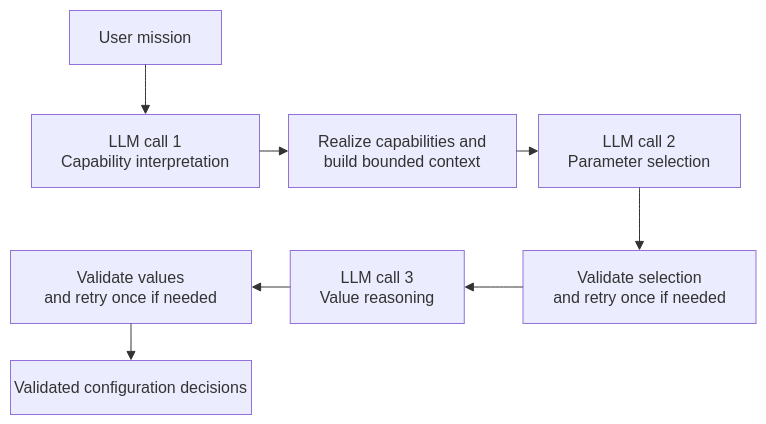
\includegraphics[width=0.72\textwidth]{pics/three_call_llm_pipeline.png}
    \caption{Three-stage language-model reasoning pipeline with deterministic processing between calls.}
    \label{fig:three-call-llm-pipeline}
\end{figure}

The capability interpreter receives the user's mission and a language-model-safe projection of the capability registry. The registry represents human-authored robot design knowledge: supported capabilities, available implementations, descriptive characteristics, and dependency information. It does not expose concrete renderer assignments to the language model. The model therefore decides what capability the user requested, not how launch files should be manipulated.
The interpretation is sparse. For each supported capability, the model may mark it as enabled, explicitly disabled, or unmentioned. When enabled, it may select a supported implementation if the request justifies a specific choice. Unmentioned and disabled are deliberately different states. An unmentioned capability preserves the baseline and creates no override. An explicitly disabled capability produces a deterministic request to disable the components belonging to that capability.
The interpreter can also return terminal outcomes. An unsupported outcome indicates that the request cannot be expressed using the available robot capabilities. A clarification outcome indicates that information required for a material decision is missing. Terminal outcomes stop the pipeline before configuration generation.
After schema validation, capability choices are expanded using the full registry. Dependency requirements are applied, conflicting capability or implementation choices are rejected, and component claims are merged deterministically. The result records active components, selected implementations, displaced implementations, required connections, concrete launch-level realization values, and provenance explaining why every claim exists.
The capability registry is validated against the frozen system before mission processing. Its component identifiers must refer to known deployed components, its realization keys must exist in the physical configuration representation, its connection endpoints must be known, and its wiring references must exist. Dependency cycles, unknown implementations, duplicate claims, and inconsistent component families are rejected before a mission is interpreted.
The realization method is intentionally bounded to the supported robot rather than formulated as a universal component-selection solver. It applies explicit capability dependencies and conflicts declared by the robot designer in order to preserve deterministic behavior. 
Required connections declared by the selected implementations are resolved against the unified system model. The method checks source and target components, publisher and subscription roles, effective names, interface types, wiring bindings, and known quality-of-service policies.
A locally known missing endpoint, incompatible interface type, unresolved required binding, or known quality-of-service incompatibility invalidates the realization. A connection involving an opaque external component may be classified as partially verified rather than falsely confirmed. The output is a mission-specific orchestration plan describing active deployment components and the verification state of required connections.
Capability realization does not filter the parameter space to active components. The complete physical configuration representation remains available because a mission may intentionally configure an implementation while enabling it, may change hardware values shared by several components, or may refer explicitly to an inactive component. Each catalogue record combines deterministic configuration facts with grounded source and system evidence.
All catalogue records remain candidates in principle, but they are not all inserted into one language-model prompt. A deterministic retrieval stage first constructs a bounded candidate set.
The mission text and searchable parameter fields are normalized and tokenized before scoring. Each parameter becomes a searchable document whose fields depend on the selected context variant.
Candidate ranking uses weighted lexical matching with inverse document frequency. Let $q$ denote the set of query tokens, $f$ a searchable field, and $p$ a parameter record. The lexical score can be summarized as

\begin{equation}
S(p,q)=\sum_{t \in q}\sum_f
w_f \cdot \operatorname{idf}(t) \cdot
\left(1+\log c_{p,f}(t)\right),
\end{equation}

where $c_{p,f}(t)$ is the number of occurrences of token $t$ in field $f$, and $w_f$ gives greater importance to discriminative fields than to generic text. In the semantic configuration, aliases have weight 2.5 and example user expressions have weight 2.0; an exact alias phrase, parameter identifier, or source name receives an additional exact-match bonus. The ranking is deterministic: the same frozen mission-specific catalogue, request, and retrieval configuration produce the same candidate order.
The highest-ranked candidates are retained up to a configured limit. Under the \texttt{graph} and \texttt{metadata\_graph} variants, the method then follows eligible explicit parameter relationships and shared wiring bindings for a bounded number of hops. Graph neighbors receive a discounted score and retain the identifier of the candidate through which they were discovered. This allows a lexical match for one occurrence of a shared concept, such as wheel radius, to introduce another physically related occurrence when both consuming components are active, even when the second record shares fewer words with the request.
Lexical retrieval is intentionally a transparent baseline rather than a claim of full semantic search. It searches semantically meaningful fields, but the matching operation itself remains token based. The language model performs semantic selection only after this deterministic candidate construction.
Retrieved records are serialized in rank order under a fixed character budget. The context records which identifiers were included, which candidates were omitted because of the budget, how each record was retrieved, and which relationship edges are relevant.
This bounded construction provides a reproducible context window and a measurable retrieval boundary. If a correct parameter is absent from the supplied context, the failure can be attributed to retrieval rather than to parameter selection.
The parameter-selection model receives the original mission, the complete compact metadata for each bounded candidate, a concise summary of the decided capabilities and active components, relevant wiring bindings, and a strict structured-output contract. This call uses a 16384-token context window, while capability interpretation and value reasoning retain the 8192-token setting. It must either select one or more supplied parameter identifiers or return a terminal status indicating no parameter change, unsupported intent, or a need for clarification.
For a valid selection, the model returns each selected parameter identifier together with a concise relevance explanation and, when available, identifiers for the grounding evidence it used. Deterministic validation rejects identifiers absent from the supplied context, duplicate identifiers, and evidence references that were not provided for that parameter. The language model therefore cannot introduce a parameter directly from the full catalogue or fabricate a source citation.
Value reasoning is invoked only after a valid selection. It receives the original mission, the validated selection, the selected parameter records, their current values, their known constraints, and relevant relationships. It does not receive the full catalogue. Its task is to propose a new value for each required parameter and give a concise, externally verifiable reason.
Separating selection from value reasoning prevents the model from hiding an incorrect parameter choice inside an otherwise plausible numerical answer. It also permits independent evaluation of whether the system found the right configuration elements and whether it derived the right values.
The value stage may return a clarification or unsupported result if the selected context does not contain enough information to determine a responsible change. For a valid result, every proposed change must repeat the current value observed in the frozen catalogue. This old-value check prevents a response generated against stale context from being applied silently.

\begin{figure}[htbp]
    \centering
    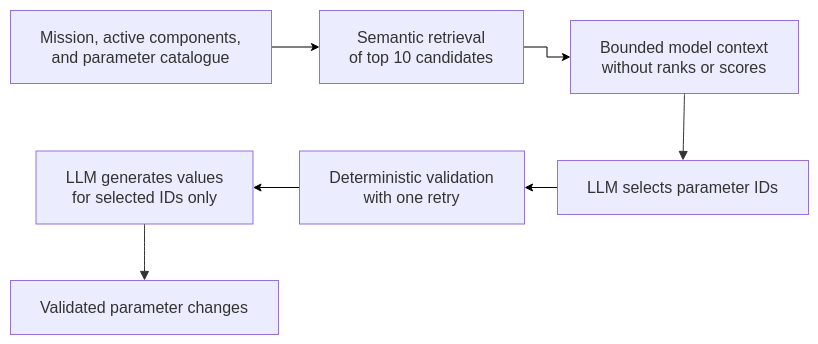
\includegraphics[width=0.90\textwidth]{pics/4parameter_retrieval.png}
    \caption{Bounded parameter retrieval followed by separated selection and value reasoning.}
    \label{fig:parameter-retrieval-reasoning}
\end{figure}

\section{Configuration Plan Generation and Validation}
\label{sec:plan-validation}
The conclusions of the language-model stages are not applied directly to files. They are converted into explicit intermediate plans that form a deterministic boundary between inference and system modification.
The first intermediate representation is the system realization produced from capability choices. It contains component activation claims, selected implementations, dependencies, required ROS connections, launch-level realization values, and provenance. The second representation is the validated set of parameter changes produced after selection and value reasoning. These two sources are merged into one sparse configuration plan.
The plan is sparse by design. It contains only values that differ because of the current mission. Unmentioned capabilities, unchanged parameters, and unrelated baseline values are not copied into it. Sparsity makes the causal effect of the request visible and reduces the risk that a model-generated response accidentally rewrites the complete configuration.
Every planned value is addressed by a canonical identifier from the physical configuration representation. Capability realization and parameter reasoning may target the same identifier only when they agree on the value. If, for example, capability realization requires an implementation to be enabled while parameter reasoning proposes disabling its launch argument, the plan is rejected instead of resolving the conflict through update order.
The plan also retains evidence and provenance. Capability values record which selected or required capability produced them. Parameter values retain the user's request and the model's concise justification. This information supports audit, failure analysis, and user-facing explanation without requiring access to hidden model reasoning.
Introducing this representation has several methodological advantages. It prevents direct language-model file editing, establishes a stable contract for validation, allows the same plan to be rendered through different output strategies, and makes the proposed change independently inspectable before application.
Validation is distributed across the method so that each stage checks the properties for which it has sufficient information. The validator does not attempt to replace semantic reasoning with an extensive hand-written configuration policy. Instead, it verifies objective properties that can be established deterministically.
At application start-up, the system model, physical configuration representation, renderer manifest, and parameter evidence are checked for supported schema versions. The evidence artifact contains hashes of the system and configuration models from which it was derived. A mismatch marks the artifact as stale and prevents its use.
The capability registry is cross-validated against these artifacts. Component identifiers, implementation references, realization keys, required connection endpoints, and wiring bindings must resolve. Dependency cycles and inconsistent declarations are rejected before mission processing.
Every language-model output must conform to its structured response contract: capability selections may contain only supported capability and implementation values, sparse-state invariants prevent an implementation from being named unless its capability is enabled, parameter selection is constrained to identifiers and evidence supplied in the bounded context, and value reasoning cannot introduce a parameter that was not selected or propose a value inconsistent with the parameter's declared type, allowed values, or known bounds. These checks establish that the model's result is grounded in the current retrieval output and the frozen catalogue; they do not assert that its semantic choice is correct. Section~\ref{sec:config-gen-validation} details how each of these checks is implemented.
Where multiple effective parameter occurrences are controlled by one physical slot, the slot representation prevents divergent proposals by construction. Where separate physical slots are related, the relationship is supplied as reasoning context and can be evaluated as part of the task annotation; the system does not impose a universal rule that every semantically related parameter must always have the same value.
The merged plan is checked against the complete physical configuration representation and the renderer interface. Every key must exist and be renderable. Capability and parameter claims targeting the same key must agree. The plan remains sparse, but the resolved rendering context must become complete after it is overlaid on the baseline. Generated artifacts then pass structural checks and, optionally, a more expensive offline equivalence analysis, detailed alongside the renderer implementation in Section~\ref{sec:config-gen-validation}.
These validation layers establish structural and factual correctness. They do not claim to prove that every semantically plausible parameter change is physically safe for every robot or environment. Such domain assurance requires additional system-specific constraints or experimental validation.

\begin{figure}[htbp]
    \centering
    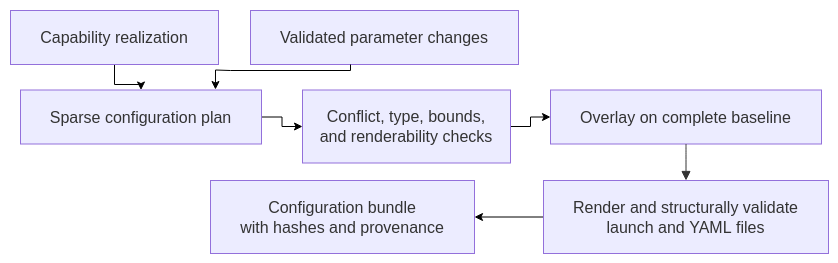
\includegraphics[width=0.90\textwidth]{pics/sparse_plan_validation.png}
    \caption{Validation and deterministic application of the sparse configuration plan.}
    \label{fig:sparse-plan-validation}
\end{figure}

\section{Configuration Application and End-to-End Workflow}
Once the sparse plan has passed the validation described in Section~\ref{sec:plan-validation}, it is overlaid on the complete baseline and materialized through the predefined launch and parameter templates introduced above; the language model never produces launch syntax, YAML structure, output paths, or installation targets. Application produces a mission-specific launch wrapper, parameter files, a record of resolved values and merge provenance, a manifest of generated files, and structural validation results. The method stops at artifact production: it does not start ROS~2 nodes, install packages, or claim that generated behavior has been validated on a physical robot, and Section~\ref{sec:config-gen-validation} details the renderer implementation.

Consider the request: ``Build a map using KISS-ICP and limit its range to 20 metres.'' This request combines a high-level capability choice, an implementation choice, and a lower-level algorithm parameter change, making it representative of the complete method and showing how the stages defined in the preceding sections act together.

Before the request is processed, the repository has already been analyzed: the frozen system model identifies the deployed mapping, laser, odometry, and conversion components, and the capability registry declares mapping and odometry as supported capabilities with KISS-ICP as one available odometry implementation.

The capability interpreter maps ``build a map'' to the mapping capability and ``using KISS-ICP'' to the KISS-ICP odometry implementation; it does not attempt to turn ``20 metres'' into a capability, leaving that phrase for the parameter-reasoning stages. Deterministic realization then activates mapping, activates KISS-ICP together with the laser-scan-to-point-cloud conversion it requires, displaces the alternative kinematic ICP implementation, and checks the resulting sensor-to-odometry chain against the frozen system model; a confirmed structural incompatibility would stop the request before parameter reasoning.

Bounded retrieval ranks the complete catalogue using the mission terms, so records associated with the KISS-ICP range are expected to rank highly. The selection model receives only this retrieved context and selects the maximum-range parameter -- and only that parameter, not unrelated mapping frequencies, frame names, or topic parameters -- because the request explicitly limits the implementation's sensing range. The value model then receives the selected record, its current value, type, and constraints, and proposes a new value of 20 metres, explained as directly stated by the user; the reported old value and the new value are checked against the frozen catalogue as described in Section~\ref{sec:plan-validation}.

The validated parameter change is merged with the launch-level values from capability realization into a sparse plan containing only the values needed to activate mapping, select KISS-ICP and its dependency, displace the alternative implementation, and set the requested maximum range. After the checks described above, the plan is overlaid on the complete baseline and rendered; the resulting files are checked structurally and packaged with traceability information. At no point does the language model directly edit a ROS file or select an output path.

This example illustrates the intended division of responsibility: the language model maps natural language to supported capabilities, relevant parameters, and requested values; deterministic representations establish what exists; deterministic realization expands robot-specific design knowledge; and deterministic validation and rendering ensure that the conclusion can be applied to the modeled system.

\begin{figure}[htbp]
    \centering
    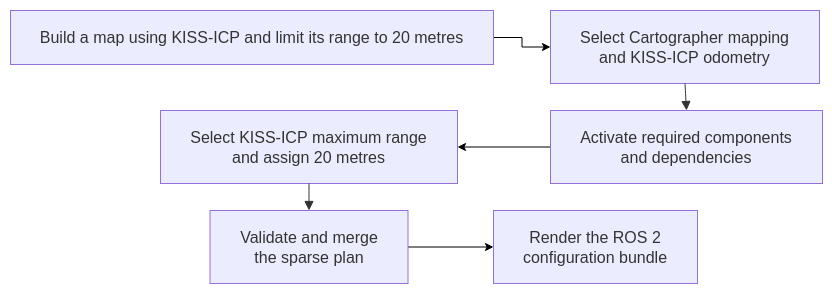
\includegraphics[width=0.90\textwidth]{pics/end_to_end_request.png}
    \caption{Processing of a representative mapping and KISS--ICP configuration request.}
    \label{fig:representative-end-to-end-request}
\end{figure}

\section{Limitations and Design Boundaries}
The proposed method intentionally adopts several boundaries in order to keep the research focus on source-grounded language-model reasoning.
First, static analysis is incomplete by nature. Dynamically generated node names, reflective Python behavior, runtime-created interfaces, environment-dependent substitutions, and unsupported language patterns may remain unresolved. The method exposes these limitations explicitly but cannot infer facts absent from the analyzed repository.
Second, external ROS packages may appear in launch descriptions without locally available source code. Their deployment presence can be represented, but their internal parameters and interfaces cannot be validated to the same degree as local components. Connections involving such packages may remain partially verified until runtime information or additional package models are provided.
Third, the capability registry is human-authored robot design knowledge. The method validates its references and internal consistency, but it does not discover autonomously which high-level capabilities a robot should support or which implementation combinations are desirable. The registry is deliberately small and robot-specific rather than a universal ontology of ROS functionality.
Fourth, the retriever remains lexical even when language-model-generated metadata is enabled. It searches deterministically extracted fields together with frozen descriptions, aliases, example user expressions, and semantic relationships, but candidate matching still depends on normalized token and phrase overlap. Incorrect or incomplete enrichment can therefore mis-rank a candidate, while a concept absent from every searchable field may still be missed. Embedding, hybrid, or learned retrieval can be evaluated later as separate methods, but they are not silently assumed by the proposed method.
Fifth, structural validation cannot guarantee physical safety or behavioral success. Type correctness, known bounds, valid ROS names, and compatible interfaces are objective checks; deciding whether a change is appropriate for a particular robot, environment, or safety envelope may require additional domain constraints, simulation, or hardware experiments.
Sixth, the method produces deployable configuration artifacts but does not itself launch, monitor, or recover the ROS~2 system. Runtime lifecycle management, distributed deployment, fault recovery, and automatic rollback are outside the proposed configuration-reasoning boundary.
Finally, structured generation cannot eliminate semantic errors; bounded context, validation, abstention, and deterministic application limit their consequences.
